\documentclass[a4paper,12pt]{report}
\usepackage[utf8]{inputenc}
\usepackage[right=30mm,left=30mm]{geometry}
\usepackage{microtype}
\usepackage[T1]{fontenc}
\usepackage{natbib}
\usepackage[francais]{babel}
\usepackage[Bjornstrup]{fncychap}
\usepackage{amssymb}
\usepackage{amsmath}
\usepackage{amsfonts}

\usepackage{xspace}

\usepackage{fourier}
%\usepackage{lmodern}

\usepackage{textcomp}

\usepackage{graphicx}
\usepackage{hyperref}
%\usepackage{pdflscape} %% mettre une page au format portrait (landscape)
\usepackage{xcolor}
\hypersetup{
	colorlinks=true,
	breaklinks=false,
	urlcolor= blue,
	linkcolor= blue,
	citecolor= blue}
\frenchbsetup{
	CompactItemize=false,         % ne pas compacter les listes
	%ThinSpaceInFrenchNumbers=true % espace fine dans les nombres
}
\usepackage[mediumspace,mediumqspace,squaren]{SIunits} %utilisé pour les unités (micromètre)
%\usepackage[options]{natbib}: citation en chifres dans le texte.

\newcommand{\Ctreize}{$\delta$\textsuperscript{13}C\xspace}

\newcommand{\Odixhuit}{$\delta$\textsuperscript{18}O\xspace}

\date{Québec, le 19 avril 2018}
\begin{document}
	
	\begin{titlepage}
		\begin{center}
			
			
\includegraphics[height=2.4cm]{logo_laval} \hspace{2.9cm}
			
\includegraphics[height=2.6cm]{crmr_logo}
			
			\vspace{\fill}
			
			\begin{center}
				\Huge Modélisation des effets des conditions climatiques sur les propriétés du bois
			\end{center}
			
			\hrule height 1pt
			
			\begin{flushright}
				\Large André \bsc{Soro}
			\end{flushright}
			
			\vspace{\fill}
			
			\Large Directeur : Alexis \bsc{Achim} \\ Co-directeur : Patrick \bsc{Lenz}
            \date{19 avril 2018}
		\end{center}
	\end{titlepage}
	
	\tableofcontents
	\listoffigures
	


%\part*{Introduction et problématique}
\chapter{Introduction et problématiques}
%\phantomsection\addcontentsline{toc}{chapter}{Introduction} % inclure dans TdM

L'épinette blanche (\textit{Picea glauca} (Moench) Voss) est une espèce d'arbre qui a une grande importance dans les forêts du Québec et plus largement du Canada. Elle a une valeur économique importante du fait de sa distribution géographique et de son abondance (Figure~\ref{fig:distribution}). Le bois d'épinette est apprécié comme bois de construction, comme matériel pour des produits de menuiserie et pour la mise en pâte grâce aux caractéristiques de ses fibres \citep{Zhang2008}. Ainsi, l'épinette blanche est fortement reboisée dans  divers systèmes sylvicoles au Canada. Cette espèce présente une certaine plasticité, car elle est capable de s'adapter à divers types de sols et conditions climatiques \citep{Nienstaedt1990}. Les propriétés physiques du bois d'épinette sont principalement liées à son anatomie \citep{Rossi2012}. Les variations de certains caractères anatomiques du bois tels que la largeur des cernes et de certaines de ces propriétés physiques, notamment sa densité, dépendent de l'activité cambiale (activité du cambium), qui elle est régie par deux conditions principales: génétiques et environnementales \citep{Dufour2010,Rossi2012}. La densité est un caractère important pour la qualité du bois et elle est influencée par l'épaisseur de la paroi et le diamètre cellulaire. Elle est donc influencée indirectement par les caractères anatomiques. L'activité cambiale, quant à elle, influence strictement le nombre de cellules formées (largeur de cerne) et d'autres facteurs comme la durée de vie des initiales va déterminer entre autres l'épaisseur de la paroi lors de la maturation cellulaire.\\

Depuis les années 1950, plusieurs études se sont intéressées à la variation génétique et phénotypique de la croissance de l'épinette blanche et des caractéristiques de son bois \citep{Corriveau1971,Li1993,Li1997}. Initialement, les programmes d'améliorations génétiques s'intéressaient principalement à la croissance rapide des arbres et visaient ainsi à augmenter la croissance en volume des plantations futures. Cependant, les  propriétés mécaniques et l'anatomie du bois étaient peu considérées dans ces programmes de façon générale \citep{Zhang1995}. Ce n'est que récemment que des recherches se sont intéressées à l'évaluation des variations génétiques des propriétés (mécaniques) du bois, telles que la densité du bois, la longueur des fibres et leur impact sur la production du bois \citep{Hernandez2001,Beaulieu2003}. De plus en plus d'études se penchent sur la génétique des propriétés radiales du bois telles que la densité, la rigidité du bois, la résistance à la flexion et l'angle des microfibrilles \citep{Lenz2010,McLean2016}. Ces études ont pour but d'obtenir une meilleure compréhension du contrôle génétique de ces caractères et les possibilités d'inclure la qualité du bois comme critère de sélection dans les programmes d'amélioration génétique. C'est dans cette optique que \cite{Lenz2011} ont étudié les relations entre les propriétés du bois notamment la densité, l'angle des microfibrilles et le module d'élasticité ainsi que la croissance radiale chez \textit{Picea glauca}. Les auteurs ont trouvé que le niveau de corrélation entre les propriétés du bois est variable en fonction de l'âge cambial, donc elle varie du bois juvénile au bois mature. Leurs travaux ont montré une absence de corrélation entre (1) l'angle des microfibrilles et la densité du bois, (2) l'angle des microfibrilles et les propriétés liées à l'anatomie des fibres telles que leur diamètre et (3) l'angle des microfibrilles et l'épaisseur de la paroi. \\ 

\begin{figure}
	
	\centering
	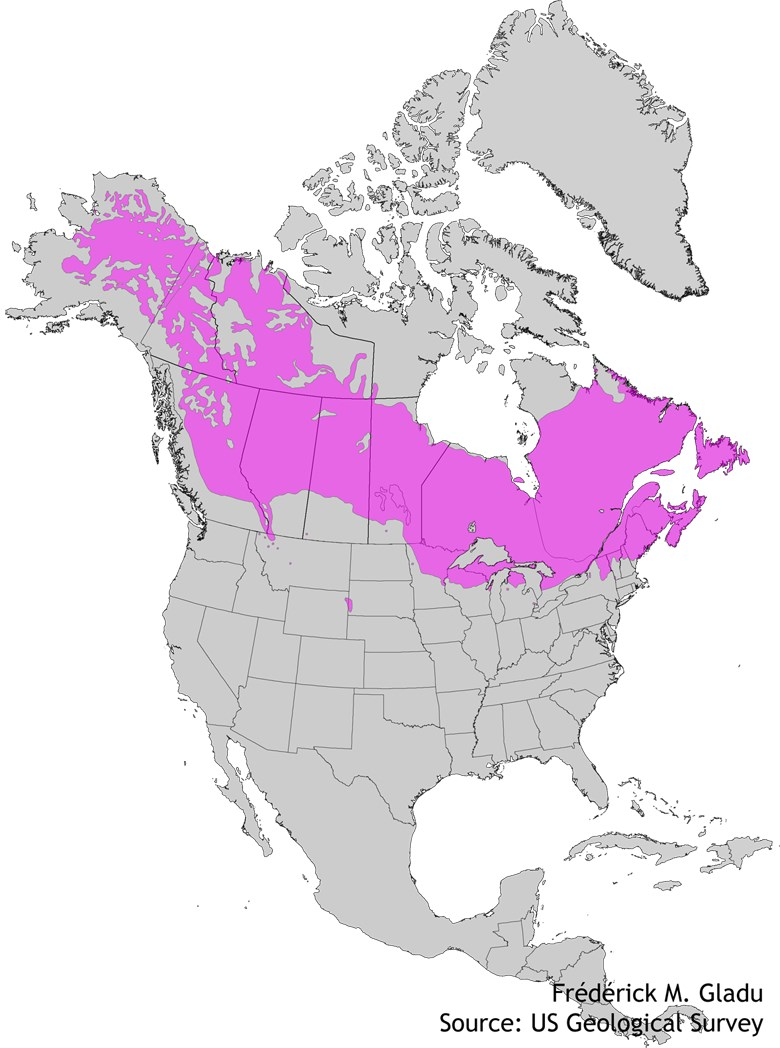
\includegraphics[width=0.65\textwidth]{distribution.jpg}
	\caption{Distribution de l'épinette blanche au Canada}
	\label{fig:distribution}
	
	
\end{figure}


\cite{Ivkovich2002} ont trouvé une relation entre différents caractères anatomiques du bois d'épinette, notamment l'angle des microfibrilles, et la densité à l'aide de carottes prélevées à hauteur de poitrine (DHP). Dans leur étude, ils ont observé que l'analyse des composantes anatomiques n'apporte pas un avantage précis pour contourner la relation négative qui existe entre la croissance et la densité du bois. D'autres études ont mis en évidence un lien entre la densité du bois, la rigidité en flexion et la résistance mécanique du bois scié \citep{Saranpaa1994,Alteyrac2006}. Ces résultats soulignent le caractère clé de la densité parce qu'elle est l'un des indicateurs de la qualité du bois les plus largement utilisés. Ainsi, elle affecte la performance du bois scié, l'aptitude à la fabrication de panneaux et les rendements en pâte \citep{Macdonald2002}. La densité du bois influence aussi le calcul des valeurs calorifiques pour les applications de biomasse pour la bioénergie \citep{Mckendry2002}. Elle peut être variable au sein d'une même espèce en lien avec les conditions environnementales (climat, compétition, densité du peuplement etc.) ou la famille. Par conséquent, les modèles de prédiction de la densité du bois devraient combiner l'âge cambial, la génétique et les conditions environnementales. L'importance de la densité pour la qualité du bois est la raison pour laquelle nous nous intéresserons à ce caractère dans notre étude. \\

Au Québec, les prochaines sélections génétiques dans les programmes d'amélioration des différentes espèces d'épinettes considéreront l'héritabilité des propriétés du bois \citep{Mullin2011, Beaulieu2009}. Par définition, l'héritabilité est une donnée statistique qui sert à évaluer la part des facteurs génétiques et celle des facteurs environnementaux dans la construction du phénotype d'une population donnée. Alors, \cite{Lenz2010} ont étudié l'héritabilité des caractéristiques d'anatomie cellulaire du bois d'épinette blanche en fonction de l'âge cambial. Leur étude a montré que la part du contrôle génétique pour les caractéristiques d'anatomie cellulaire augmente avec l'âge cambial. Par contre, le contrôle génétique de l'angle des microfibrilles est constant. En outre, \cite{Lenz2011} ont étudié les relations génétiques entre propriétés du bois et leurs conséquences sur l'amélioration des arbres. Ces études ont montré que les propriétés du bois sont contrôlées en grande partie par la génétique. La sélection génétique pourrait donc altérer les propriétés du bois et améliorer la qualité de la fibre dans les futures plantations. Toutefois, des facteurs tels que les conditions environnementales semblent influencer les propriétés du bois et leurs effets peuvent varier en fonction du bagage génétique des arbres. Or, les interactions entre la génétique et le climat restent peu étudiées pour les propriétés du bois \citep{Housset2018}. De ce fait, il y a un besoin de mieux comprendre comment l'amélioration génétique et les variations climatiques peuvent influencer les propriétés du bois. \\

Le climat est un facteur déterminant pour la croissance et les processus physiologiques des arbres. De ce fait, les conditions climatiques affectent fortement les propriétés du bois. En effet, certains facteurs climatiques comme la sécheresse peuvent engendrer un stress chez les arbres et entraîner une variation des propriétés du bois, notamment la densité, la largeur des cernes et la conductivité. La disponibilité en eau qui est dépendante du climat, est un facteur important qui influence la croissance des arbres \citep{Lebourgeois2005}, alors un déficit hydrique est une source de stress qui affecte les processus physiologiques \citep{Waring1987}. Il est donc important de déterminer les potentiels effets des changements climatiques sur la qualité du bois et son héritabilité dans une optique de reboisement. En effet, les modèles de climat futur prévoient des changements de régime hydrique avec des périodes de dessiccation et de désaturation des sols plus importantes \citep{IPCC_2015}. Cela explique notre intérêt pour l'impact potentiel des variations climatiques sur la qualité du bois. \\

Plusieurs études antérieures se sont intéressées à l'effet des conditions environnementales sur les propriétés du bois. L'environnement (climat, disponibilité en eau, etc.) affecte directement l'activité cambiale de l'arbre \citep{FRITTS1976,Kozlowski1997}. La division des cellules cambiales étant responsable de la quantité et de la qualité du bois \citep{Begum2013}, les conditions environnementales peuvent donc influencer la qualité du bois. L'impact météorologique sur la qualité du bois varie d'un site à l'autre en fonction du type de stress auquel sont exposés les arbres. Ainsi, dans les régions où les arbres sont très exposés au vent, par exemple, ils auront tendance à former du bois de réaction. Les précipitations peuvent aussi affecter la qualité du bois dans certaines régions. \cite{Bouriaud2005} ont trouvé une forte corrélation positive entre le déficit en eau du sol et la densité du bois. Un déficit d'eau dans le sol peut ralentir la croissance, ce qui peut entraîner une augmentation de la densité du bois \citep{GARDINER2011}. En plus, l'impact climatique sur l'anatomie du bois a été montré dans plusieurs études \citep{Bouriaud2005,Fritts2001,Campelo2013}. Ces études montrent un effet du climat sur la croissance des arbres et sur la variation intra-annuelle de la densité. Dans certaines études, la variation des propriétés du bois telles que la largeur de la paroi cellulaire \citep{Fritts2001}, la croissance radiale \citep{Jyske2009}, la variabilité intra-annuelle de la densité du bois \citep{Wimmer2000,Rigling2001,Wilkinson2015} a été utilisée comme marqueur de sécheresse. Ces études ont mis en évidence que les fluctuations climatiques peuvent conduire à des variations intra-annuelles de la densité du bois. \\

La densité du bois peut avoir des variations inter et/ou intra-annuelles au sein d'un même arbre. \cite{Fritts2001}, définit les variations intra-annuelles de la densité du bois comme la présence de cellules semblables au bois initial dans le bois final et/ou la présence de cellules semblables au bois final dans le bois initial. Ces variations intra-annuelles de la densité sont induites par une variation des conditions environnementales durant la période de croissance radiale. L'activité cambiale est donc modifiée, ce qui peut fournir des informations sur les conditions climatiques \citep{Campeloa2007,Campelo2013,Novak2013}. Par conséquent, l'étude de la variation de la densité intra-annuelle permet d'avoir des informations sur l'environnement et inversement. Les variations inter-annuelles, par contre, peuvent être induites par les conditions environnementales lors de la période de croissance, de l'année précédente ou par l'activité écophysiologique annuelle \citep{Hughes1984,DArrigo1992}. Elles se définissent par une variation de la densité et/ou de la largeur des cernes d'une année à l'autre. La compréhension de la variation de la densité est alors nécessaire dans une optique d'anticipation de l'impact du climat futur sur la qualité du bois.\\

Parmi les méthodes utilisées pour la compréhension de l'effet du climat sur les propriétés du bois nous avons l'utilisation des isotopes qui prend de plus en plus d'ampleur. Les isotopes sont des nucléides qui ont le même nombre de protons, mais ayant un nombre de neutrons différent. De plus en plus d'études récentes utilisent l'analyse isotopique qui est une analyse de la structure fine (isotopes stables) du bois formé lors des événements climatiques particuliers pour faire le lien entre la variabilité des propriétés du bois telles que la largeur du cerne, la densité du bois et les conditions climatiques. La plupart des éléments chimiques contiennent plus d'un isotope stable, qui se définit comme un isotope qui ne subit pas de désintégration radioactive dans le temps \citep{West2006}. La plupart des processus biochimiques et biogéochimiques sont associés à un filtre isotopique en défaveur des isotopes lourds dans les mélanges chimiques (p.ex. \up{18}O plus que \up{16}O). Ce filtre isotopique entraîne une variation isotopique des pools de sources et de produits à différentes étapes d'un cycle biogéochimique et des ressources utilisées par les organismes de ces pools \citep{Dawson2002}. Le passage du carbone de l'atmosphère aux feuilles de la plante par la photosynthèse est un processus qui discrimine contre le \up{13}C. L'ouverture et la fermeture des stomates de la plante influencent cette discrimination. En effet, la fermeture des stomates entraîne une modification de la signature isotopique du carbone et de l'oxygène dans le bois \citep{Farquhar1993, Bigras2005}. L'air interne des feuilles est appauvri en \up{13}C par rapport à l'air ambiant, ce qui entraîne un «fractionnement dû à la diffusion». Si l'ouverture stomatique est extrêmement petite (0,1 mm), les collisions avec les cellules de garde deviennent importantes et le fractionnement est beaucoup plus élevé, mais cela ne se produit que chez les espèces avec une fréquence élevée de très petits stomates tels que les Citrus (\textit{Citrus glauca} et \textit{Microcitrus sp.}) \citep{Farquhar1993}. Une fermeture des stomates suite à un déficit d'eau peut avoir le même effet. Par conséquent, la composition des isotopes stables du carbone et de l'oxygène du bois est de plus en plus intégrée dans les travaux qui ont pour but de déduire les conditions climatiques et les réactions physiologiques des arbres \citep{McCarroll2004, Sternberg2009,Sarris2013}. \\

Les méthodes basées sur la mesure d'isotopes stables sont parmi les outils les plus précis pour la compréhension des relations entre les plantes et leur environnement \citep{Dawson2002}. Les isotopes sont inégalement répartis entre et au sein de différents composés, et cette distribution isotopique peut mettre en évidence des informations sur différents processus, notamment physiques, chimiques et métaboliques impliqués dans les transformations du carbone \citep{Farquhar1989}. L'utilisation des méthodes basées sur les isotopes de carbone stables dans le matériel végétal, et particulièrement dans les cernes annuels, s'est généralisée quand le modèle de \cite{Farquhar1989} est devenu un modèle prédictif des effets environnementaux sur les rapports isotopiques. La proportion d'isotopes stables (\Ctreize et le \Odixhuit) dans une partie de la plante varie suite aux processus physiques et biologiques. Le fractionnement isotopique ($\Delta$) est la discrimination de l'isotope lourd en faveur de l'isotope léger. Le fractionnement isotopique entre deux parties de l'arbre suite à un processus nous renseigne sur la dynamique de celui-ci \citep{Farquhar1989}. La composition en isotopes stables du bois et de la cellulose peut être utilisée pour expliquer certains mécanismes dendroclimatiques. La cellulose est le constituant principal du bois et donc le plus utilisé pour les mesures de \Odixhuit et \Ctreize dans les arbres. Le \Ctreize, le \Odixhuit du bois dans les cernes annuels peuvent refléter les conditions météorologiques subies par l'arbre \citep{Duquesnay1998,McCarroll2004,Hartl-meier2015}. Le fractionnement isotopique du carbone et de l'oxygène pendant la photosynthèse est utile pour évaluer l'impact environnemental sur les variations intra-annuelles de la densité \citep{Farquhar1989,JonLloyd1994}. Des études récentes ont montré que l'anatomie du bois couplée aux isotopes stables (\Ctreize et \Odixhuit) permettent une meilleure interprétation entre variations intra et interannuelles de la densité et la physiologie de l'arbre \citep{Micco2007,Vaganov2009,Sarris2013}. \\

Le \Odixhuit dans le bois est relié à la quantité de précipitations \citep{Bonal2000} et il existe une relation positive entre le \Ctreize et la fermeture des stomates qui elle est relié à la température et aux précipitations \citep{Pons2011}. Par conséquent, l'utilisation couplée du \Ctreize et du \Odixhuit permet une prise en compte à la fois des précipitations et de la température de l'air (conditions climatiques plus précises) dans la compréhension de la relation entre climat et signature isotopique du bois. Parmi les effets sur lesquels nous renseigne les isotopes stables, nous avons la sécheresse qui est un stress climatique pour l'arbre.\\ 

La réaction de l'arbre face à certains stress climatiques, notamment la sécheresse, peut être fonction de l'intensité de celle-ci. Afin, de prendre en compte les potentielles conséquences des changements climatiques qui selon les prévisions vont occasionner des sécheresses de plus en plus intenses et fréquentes \citep{IPCC_2015}, il est important d'inclure des données récoltées dans des conditions de sécheresse intense dans nos modèles pour une meilleure prédiction. Les expériences avec stress climatique intense et les modèles qui prennent en compte ce facteur permettront de faire des améliorations génétiques pour une production de bois de bonne qualité dans un climat changeant.\\

De façon générale, les travaux qui ont montré une relation entre la sécheresse et les propriétés du bois ont été réalisés sur des arbres qui n'ont pas subi un stress intense \citep{Xu2012,Drew2009,Campelo2013,Jyske2009,Wilkinson2015}. \cite{Wilkinson2015} ont observé un compromis négatif entre la sécurité hydraulique et l'efficacité au niveau cellulaire. Les sorties de leur modèle ont montré que la variation intra-annuelle de la densité augmente la sécurité hydraulique pendant les périodes de sécheresse. Cependant, l'effet potentiel qu'une sécheresse intense peut avoir sur la densité du bois demeure difficile à prévoir. Alors que le ralentissement de croissance associé à des sécheresses de faible intensité peut entraîner une augmentation de la densité (tel que rapporté plus haut), il est concevable qu'une sécheresse très intense puisse limiter la photosynthèse à un point tel que les ressources manquent pour produire une paroi cellulaire épaisse, et donc un bois dense.\\ 

Le bilan de la littérature met en évidence que la variation des conditions climatiques et le contrôle génétique des propriétés du bois ont été souvent étudiés séparément. Des études récentes ont trouvé une relation entre les conditions climatiques comme la sécheresse, la température et le contrôle génétique sur les propriétés du bois \citep{Housset2018, Heer2018}. Ils ont observé un lien direct entre les caractères dendroécologiques et la génétique. Ces études font un lien entre la résilience des arbres aux variations climatiques et le contrôle génétique. Par contre, la partie de ces caractères qui associée à la variabilité de la famille est très peu connue. Notre étude permettra de mieux connaître l'impact de la famille sur la réaction des arbres face aux variations climatiques, notamment à la sécheresse. Les résultats pourront être utilisés pour l'amélioration génétique et permettre d'anticiper les effets des changements climatiques sur la production et la qualité du bois. \\


\section{Objectifs}
%\phantomsection\addcontentsline{toc}{section}{Objectifs}

Ce projet a pour objectif de lier la variation des propriétés du bois au climat et d'évaluer le contrôle génétique de cette variation des propriétés aux conditions environnementales dans des populations d'épinettes blanches utilisées dans le programme d'amélioration génétique au Québec. Parmi les variations environnementales, l'étude se focalisera sur les effets des précipitations et du stress hydrique. Les propriétés du bois qui seront évaluées sont principalement la largeur des cernes, la densité du bois, l'angle moyen des microfibrilles de cellulose dans la paroi cellulaire et la proportion en isotopes stables de \Ctreize et \Odixhuit. Le projet sera élaboré en trois chapitres qui permettront la rédaction d'autant d'articles scientifiques. Les objectifs spécifiques de chacun des chapitres sont les suivants:\\

\begin{itemize} 
	
	\item Caractériser les profils de densité et de largeur des cernes afin d'identifier les familles ayant produit le bois le plus « uniforme » au cours des années, et ce, malgré les possibles variations environnementales. 
	
	\item Évaluer l'influence de différents niveaux de stress hydrique imposé artificiellement sur les propriétés du bois de jeunes semis et sur la conductivité du xylème et mesurer la variabilité de cette réaction parmi différents croisements et clones. 	
	
	\item Quantifier les effets des conditions météorologiques sur la proportion d'isotopes stables lourds ( \Ctreize et \Odixhuit) dans la cellulose du bois, puis déterminer dans quelle mesure cette proportion peut varier entre les familles analysées.
	

	
\end{itemize}

   
Dans la première partie de ce travail, la caractérisation des profils de densité et de largeur des cernes permettra de mettre en évidence les familles ou individus qui ont produit du bois relativement \og uniformes \fg au cours des années malgré les possibles variations inter-annuelles des conditions météorologiques. Les familles montrant ce type de profil (uniforme) seront considérées comme moins sensibles aux variations climatiques qui peuvent devenir plus marquées à cause des changements climatiques. Ces résultats pourront servir à la sélection d'individus ayant un bois uniforme face aux extrêmes climatiques pour les futures générations d'arbres utilisés dans les programmes d'amélioration de l'épinette blanche au Québec. Ce chapitre permettra également l'identification des facteurs météorologiques qui influencent significativement la variabilité de la qualité du bois de l'épinette blanche. Dans le deuxième chapitre, l'analyse des résultats de l'expérimentation en serre permettra de mettre en évidence l'effet de différents gradients de stress hydrique sur l'angle des microfibrilles de la cellulose dans la paroi cellulaire et la conductivité du xylème. Dans le dernier chapitre, nous nous intéresserons à la réaction des arbres face au stress hydrique à une échelle plus fine, soit l'échelle moléculaire, et mesurerons la variabilité de la signature isotopique entre les familles. \\


\section{Hypothèses}
%\phantomsection\addcontentsline{toc}{section}{Hypothèses}

Dans cette étude nous avons émis les trois hypothèses suivantes qui correspondent aux différents chapitres du projet, et qui sont relatives aux effets des conditions environnementales (principalement l'effet du stress hydrique) sur la variation des propriétés du bois :\\


\begin{itemize}	
	

	\item  \emph{L'impact d'une sécheresse sur la densité du bois dépend du moment où elle survient lors de la saison de végétation. On observe une augmentation de la densité du bois si la sécheresse survient lors de la formation du bois initial et inversement si elle arrive lors de la formation du bois final. Cependant, certaines familles d'arbres réagissent de façon moins marquée que d'autres face à ces épisodes de sécheresse, ce qui rend leur profil inter-annuel de densité plus uniforme.} \\
	
	La proportion de bois initial tend à être plus importante que celle du bois final dans les larges cernes annuels, et inversement pour les cernes étroits \citep{Moore2011} (Figure~\ref{fig:proportiondebois}). Sachant que la masse volumique (densité) du bois est minimale dans le bois initial et maximale dans le bois final, une diminution de la largeur du cerne annuel entraîne généralement une augmentation de la masse volumique de celui-ci. Toutefois, si la sécheresse arrive pendant la formation du bois final nous nous attendons à une diminution de la densité qui s'explique par une faible proportion de bois final dans le cerne annuel. \cite{Vieira2013} ont mesuré à haute résolution la croissance radiale journalière et saisonnière de la tige du pin maritime (\textit{Pinus pinaster}). Les auteurs ont observé une variation de la croissance radiale avec un profil journalier et saisonnier qui était régi par la disponibilité en eau et la température. Cette étude montre également qu'une faible teneur en eau limite la croissance radiale et entraîne une inactivité chez l'arbre (état de dormance). Cette étude soutient notre hypothèse, car elle montre que l'apparition d'un déficit en eau à un moment précis influence directement la croissance radiale à l'instant même. L'influence d'une variation des conditions climatiques sur l'activité cambiale a été observée également par la fluctuation intra-annuelle de la densité (FIAD). Cette variation de densité est une réaction à des changements dans les conditions environnementales. \cite{Vieira2015} ont étudié l'influence du climat sur la formation de FIAD dans les cernes et leurs résultats montrent qu'elles sont fortement dépendantes des précipitations. Ces études ont mis en évidence que la formation des cellules et la croissance radiale dépendent fortement des variations climatiques au cours de la saison de végétation. Au vu de ces résultats, l'on peut s'attendre à une augmentation ou une diminution de la densité du bois en cas de sécheresse en fonction du moment ou celle-ci survient.\\
	Une étude récente a mis en évidence qu'il existe une relation entre la génétique et les propriétés du bois \citep{Housset2018}. Dans cette étude, les auteurs ont combiné la dendroécologie à la génétique. Les résultats ont montré une influence du climat sur certaines propriétés du bois, mais aussi un effet de la population sur ceux-ci. Ces résultats nous font penser que la réaction des arbres face aux variations climatiques et soumis à une variation génétique peut varier varie entre différentes familles.\\
	
	\begin{figure}
		
		\centering
		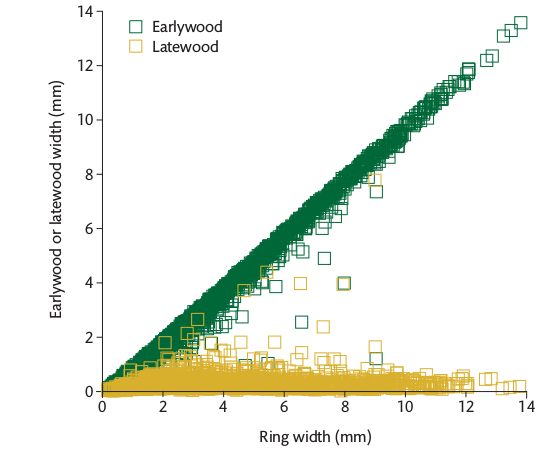
\includegraphics[width=0.65\textwidth]{wood.png}
		\caption{Largeur du bois initial et du bois final en fonction de la largeur totale du cerne chez l'épinette de Sitka \textit{Picea sitchensis}
		\citep{Moore2011}}
	    \label{fig:proportiondebois}
		
		
	\end{figure}
	

	\item \emph{ Le stress hydrique entraîne une diminution de l'angle des microfibrilles de la paroi cellulaire et affecte négativement la conductance par la fabrication de trachéides de type \og bois final \fg jusqu'à l'arrêt total de fabrication de cellules à partir d'un certain seuil de sécheresse. Une part de la variabilité des réactions observées dans ces situations peut être attribuable aux croisements et aux clones étudiés.}\\ 
	 
	Dans leur étude \cite{Xu2012} ont essayé de comprendre l'influence de la sécheresse sur l'angle des microfibrilles. Cette étude a mis évidence le fait qu'une augmentation de la température entraîne une diminution de l'angle des microfibrilles alors qu'une augmentation des précipitations a l'effet inverse. Leurs travaux offrent une perspective quant à la reconstitution du climat passé par l'étude de l'angle des microfibrilles qui, selon leurs résultats, est plus précise que l'utilisation de la largeur des cernes. En effet, les travaux ont montré que 60\% de la variabilité de l'angle des microfibrilles est expliqué par le climat, contre 37\% de la variabilité de la largeur des cernes chez l'épinette. Des résultats similaires ont été observé chez d'autres espèces d'arbres. Dans l'étude de \cite{Wimmer2002}, les résultats montrent un angle des microfibrilles plus faible chez les arbres soumis à une sécheresse sévère. Les auteurs de cette étude ont soumis une population d'Eucalyptus nitens (Deane et Maiden) à différents régimes d'irrigation pendant deux saisons de croissance.\\
	
	La sécheresse affecte la disponibilité en eau du sol et la température de l'air qui à leur tour entraînent une modification de la conductance stomatique. \cite{Irvine1997} ont étudié l'impact de la sécheresse sur la physiologie du pin sylvestre (\textit{Pinus sylvestris L.})%. les auteurs
	et ont observé qu'elle est associée à une diminution du taux de transpiration. Les résultats de ces travaux montrent que le pin sylvestre modifie sa conductance stomatique pour éviter le développement d'une embolie du xylème. Cette étude a été réalisée en milieu naturel, par contre peu d'études ont observé ce phénomène dans le cas d'une expérience artificielle avec une sécheresse intense. Notre étude permettra de mieux comprendre cette réaction des semis face à un stress hydrique intense bien isolé.\\
	
	 La sécheresse étant un phénomène inconstant en milieu naturel, il est difficile de l'isoler avec précision comme facteur explicatif de la variation des propriétés du bois. Il ressort de la bibliographie que la variation de l'effet de la sécheresse sur les propriétés du bois entre clones et croisements est peu connue. En plus, l'interdépendance entre la sécheresse, l'angle des microfibrilles et les propriétés fondamentales du bois n'a pas été modélisée explicitement. Les conditions de sécheresse étant rares au Québec, nous avons choisi d'induire artificiellement des changements de conditions hydriques qui devraient avoir des impacts sur l'angle des microfibrilles et la conductance du xylème. Ce choix permettra de faire un pas en avant plus rapidement dans la compréhension des effets de la sécheresse sur les propriétés du bois.\\
		
	Notre approche permettra alors de faire varier suffisamment les conditions hydriques pour mesurer une étendue complète des réactions possibles, et ce, jusqu'à l'arrêt de la croissance. Par ailleurs, puisque l'angle des microfibrilles varie avec l'âge cambial \citep{Lindstrom1998}, l'utilisation d'arbres juvéniles pourrait expliquer une partie de la variabilité de l'angle des microfibrilles chez les semis d'épinette blanche. Dans l'expérience qui sera mise en place pour cette partie, nous nous affranchirons autant que possible de cet impact potentiel en étudiant un seul cerne annuel et en effectuant notre échantillonnage dans le bois opposé au bois de réaction produit par des semis dont les tiges sont inclinées, une stratégie déjà utilisée dans d'autres études \citep{Apiolaza2011}.\\  
	
	\item \emph{Une part significative de variabilité de la relation entre la proportion d'isotopes stables (\Ctreize et \Odixhuit) dans la cellulose du bois et les conditions météorologiques est associée à des différences entre les croisements.} \\ % Ça me convient comme hypothèse pour le moment, mais lors de la présentation de ton proposé je te demanderai d'y inclure un lien avec les propriétés du bois
	
	%AA: tout le paragraphe qui suit n'est qu'une répétition de ce que tu avais plus haut. Réduis au minimum les répétitions. J'ai essayé d'aider un peu avec quelques changements, mais je ne peux plus grand-chose à ce stade. Il s'agit pour le moment de ton hypothèse la plus faible et je pense que c'est parce qu'elle n'intègre pas les propriétés qui déterminent la qualité du bois.
	
	La photosynthèse est un processus bioénergétique qui affecte la formation des trachéides. Elle permet la synthèse de sucres à partir du dioxyde de carbone et de l'eau qui sont acheminés jusqu'au cambium pour la production de cellulose. Ces sucres sont marqués par différentes proportions d'isotopes stables à différentes étapes de leur cheminement. Le fractionnement isotopique nous renseigne ainsi sur le lien entre le climat et les propriétés du bois. La sécheresse entraîne une fermeture des stomates \citep{Farquhar1989, Farquhar1993, Nicolas2017} qui elle engendre une modification des échanges entre les feuilles et l'atmosphère et peut provoquer une augmentation de la proportion d'isotopes stables lourds (\Ctreize et \Odixhuit) \citep{McCarroll2004,Skomarkova2006,Vaganov2009,Cernusak2015} dans la cellulose du bois. La proportion d'isotopes stables peut 
	être utilisé comme une variable de prédiction de l'impact du climat future sur les propriétés du bois. Des études ont déjà fait le lien entre les conditions climatiques et la signature isotopique. C'est le cas de  \cite{Seftigen2011} qui ont remarqué dans leurs travaux une augmentation de la proportion d'isotopes stables lourds (\Ctreize et \Odixhuit) lorsque la température croit et que les précipitations diminuent.\\
	
	Les études précédentes mettent en évidence la relation qui existe entre la proportion d'isotopes stables et les propriétés du bois. Cependant, nous n'avons pas trouvé de travaux faisant le lien entre la signature isotopique, le climat et les familles. Cette partie de notre étude permettra alors de comprendre la part de variabilité de la signature isotopique dans des conditions climatiques données qui est attribuable à des différences entre les familles. 
	
	
\end{itemize} 


\chapter{Chapitre 1: Caractérisation des profils de densité et de la largeur des cernes et identification des familles avec le bois le plus « uniforme » face aux variations climatiques}


L'objectif de ce chapitre est d'identifier les familles d'arbres qui montrent des réactions moins marquées aux écarts climatiques, et qui produisent donc le bois le plus uniforme. Nous utiliserons pour cela des données de dendrochronologie et climatiques. Les données ont été récoltées sur des arbres d'épinette blanche (\textit{Picea glauca}) plantées dans le cadre d'une série de tests de sélection génétique. 


\section{Matériel et méthode}
%\phantomsection\addcontentsline{toc}{section}{Matériel et méthode}

\subsection*{Site et matériel}\label{matériel}

Le matériel utilisé dans cette étude est issu de sélection génétique pour une série de tests en fonction des provenances ou de la région géographique \citep{Beaulieu1996}. Le programme d’amélioration est mené par le Ministère des Forêts, de la Faune et des Parcs de la province du Québec. Les tests génétiques ont été mis en place à partir de semis d'épinette blanche (\textit{Picea glauca} (Moench) Voss) cultivés en pépinière et plantés à l'âge de 2 ans. L'un des sites est situé près de Saint-Casimir, au Québec, dans la zone écologique de l'érablière à tilleul, et l'autre près de Cabano (Asselin), au Québec, dans le domaine de la sapinière à bouleau jaune. Cette série d'essais a été établie en 1999 par le Service canadien des forêts et elle représente l'une des trois parties essentielles du programme d'amélioration de l'épinette blanche au Québec. Les essais ont été réalisés par blocs, dans lesquels chaque famille était représentée par cinq arbres dans une rangée-parcelle. L'espacement entre les arbres était de 2 mètres en disposition orthogonale. Les échantillons utilisés dans ce travail ont été récoltés sur 93 familles, 2500  individus environ, 1250 arbres environ / site. Les mesures de densité, de la largeur des cernes et de l'angle des microfibrilles ont été prises à hauteur de poitrine (1,3 m du sol) dans la tige de chaque arbre échantillonné. Les carottes utilisées pour les différentes mesures ont été prélevées en 2014-2015.  \\ 

Pour vérifier la précision des datations et déterminer les cernes manquants, nous avons utilisé COFECHA qui est un programme de dendrochronologie et qui sert à la datation croisée et au contrôle de la qualité des mesures sur les cernes annuels \citep{HOLMES1983}. Ainsi, comme la séparation des cernes annuel avait été effectuée par un algorithme, nous avons éliminé les échantillons (127 échantillons) dont la datation n'était pas correcte et ne pouvait pas être modifiée. % Le "pas correct" sera à préciser lors de ta présentation

\subsection*{Détermination de la densité}\label{densité}
La densité du bois a été mesurée sur des disques avec 2 rayons par disque. Les disques ont été prélevés à une hauteur de 1,3 mètre sur la face Nord. Les échantillons de carottes ont ensuite été extraits au Soxhlet avec de l'acétone pendant une nuit, puis coupés avec précision à 1,68 mm d'épaisseur à l'aide d'une scie pneumatique à deux lames, et laissés à 7\% d'humidité avant l'analyse de densité.\\
 
Tous les échantillons ont ensuite été scannés de la moelle à l'écorce par densitométrie à rayons X (Quintek Measurement Systems, TN) à une résolution de 0,0254 mm, et les données sont rapportées en tant que densité relative sur une base de poids sec. % AA: Il te faudrait aussi donner la teneur en humidité pour le volume. Normalement on utilise la densité basale qui est la masse anhydre sur le volume saturé.

%AS : Je n'ai pas cette information dans le descriptif de la méthodologie que j'ai reçue. Il faut que je demande à Patrick s'il a l'information.

\subsection*{Données climatiques}
Les données climatiques (la température et les précipitations) ont été générées par le logiciel BioSim. BioSIM est un logiciel conçu pour aider à l'application de modèles de simulation axés sur la température et les précipitations \citep{Regniere2014}. Les intrants qui ont été fournis à BioSIM pour qu'il puisse faire les simulations relatives à la température et aux précipitations sont les données de latitude, de longitude et d'altitude de chaque site d'étude. Ainsi, BioSim utilise les données des stations météo les plus proches autour de chaque site d'étude pour générer les données climatiques du site. Les stations météorologiques sont utilisées dans le calcul avec des pourcentages pondérés qui sont proportionnels à la distance de la station par rapport à la localisation du site.\\ 

Le lien entre les données météorologiques et la largeur des cernes sera fait à l'aide du logiciel DENDOCLIM2002 complété par des modèles statistiques. Dendoclim permet de calibrer la chronologie des cernes par rapport aux données climatiques en utilisant des fonctions de corrélation et de réaction. Il permet de mettre en évidence la corrélation entre cernes et climat \citep{Biondi2004}. 

\subsection*{Analyses statistiques}
Plusieurs données ont été récoltées sur les arbres des deux sites d'étude. Dans le cas de ce chapitre, nous utiliserons la densité du bois et la largeur des cernes annuels comme propriétés du bois. Concernant les paramètres environnementaux, nous utiliserons principalement les températures moyennes mensuelles et les précipitations moyennes mensuelles. Le choix de la résolution mensuelle pour les paramètres environnementaux est basé sur ce qui a déjà été fait dans d'autres études \citep{Franceschini2017}. Dans notre analyse, nous mettrons en relation la densité du bois et la largeur des cernes avec les facteurs climatiques. \\

Nous utiliserons des modèles linéaires mixtes pour nos analyses afin d'identifier les familles qui ont la densité et la largeur des cernes la plus uniforme au cours des années. Nos données contiennent des variables fixes et des variables aléatoires, ce qui explique le choix d'utiliser des modèles mixtes.\\ 
Les variables dépendantes seront la densité et la largeur des cernes. Les variables à effet aléatoire seront les facteurs site, bloc et arbre. Les variables à effet fixe seront les précipitations, les indices de sécheresse et les croisements. Nous nous servirons du logiciel R \citep{R2018} et plus spécifiquement du package NLME \citep{NLME2018} pour la construction de nos modèles linéaires ou non linéaires mixtes. Deux modèles seront construits, un modèle pour le bois initial avec les données environnementales du printemps et un deuxième pour le bois final avec les données de l'été.

% Par contre, il faut voir qu'un mois est une limite arbitraire, et qu'en plus, les mois d'une même année sont autocorrélés. Il faudra donc raffiner les analyses afin d'éviter ces problèmes.

\section{Résultats attendus}
%\phantomsection\addcontentsline{toc}{section}{Résultats attendus}

Nous nous attendons à avoir dans nos résultats des familles ayant des propriétés (largeur des cernes et densité) plus "uniformes", donc moins sensibles à la variabilité de la température et des précipitations entre les différentes années.\\ 

Les arbres ou les familles qui ont des largeurs de cernes et ou une densité peu sensibles aux fluctuations des conditions métrologiques seront considérés comme celles qui ont des profils uniformes. Ces arbres auront donc un bois de densité plus constante que les autres d'une année à l'autre, sans forte augmentation de la proportions de bois initial pour les années avec conditions climatiques favorables et avec une décroissance moins marquée de la largeur des cernes les années sèches durant lesquelles les conditions climatiques sont moins favorables à la croissance. Dans le contexte des changements climatiques où l'on s'attend à des sécheresses plus fréquentes et sévères \citep{IPCC_2015}, nous croyons que ces familles auront des caractéristiques intéressantes pour le reboisement. Il est logique d'assumer que les arbres avec peu de variations seront résilients aux écarts climatiques, mais cette affirmation ne sera pas vérifiée dans le cadre de cette thèse. L'identification des familles produisant du bois de densité uniforme sera donc effectuée dans une optique de sélection d'une propriété avantageuse pour la transformation des produits \citep{Hernandez2001}. \\ 

Les familles d'arbres les plus sensibles auront quant à elles une variation plus importante de la largeur des cernes et de la densité du bois en lien avec les fluctuations des conditions environnementales. Les familles de cette catégorie seront considérées comme moins intéressantes pour le reboisement. En effet, pour ces familles on s'attend à, (1) une diminution du bois initial lorsqu'on a une sécheresse pendant la formation de celui-ci ou (2) une diminution du bois final si la sécheresse arrive pendant la formation du bois final.\\


\section{Conclusion}
%\phantomsection\addcontentsline{toc}{section}{Conclusion}

L'identification des familles ou individus qui ont des cernes "uniformes" malgré les variations environnementales, permettra de faire une meilleure sélection pour le reboisement au Québec et plus largement au Canada. L'amélioration génétique des forêts permettra ainsi de prendre en compte la productivité et la qualité du bois dans un contexte de climat changeant.\\

Cette partie du projet permettra de faire une sélection des familles qui serviront au reboisement. Par contre, cela reste limité si nous prenons en compte les prédictions climatiques futures dans la mesure où ces arbres n'ont pas connu des sécheresses intenses comme prévu dans les prédictions. Alors, dans le chapitre 2 de ce projet, nous prendrons en compte l'intensité et la durée de la sécheresse sur les propriétés du bois (densité, angle des microfibrilles, conductivité) par la mise en place d'une expérimentation en serre. Le chapitre 2 permettra d'évaluer l'effet de différent niveaux de sécheresse sur les propriétés du bois et sur un indice de la conductivité du xylème.



\chapter{Chapitre 2: Modélisation de l'impact d'une sécheresse plus ou moins intense sur les propriétés du bois et identification des clones aux caractéristiques avantageuses}

Les objectifs de ce chapitre sont (1) d'évaluer l'influence de différents niveaux de stress hydrique imposé artificiellement sur les propriétés du bois de jeunes semis, (2) d'évaluer l'impact de la sécheresse sur la conductivité du xylème et (3) de déterminer quels croisements et clones produisent le bois aux caractéristiques les plus avantageuses en situation de stress hydrique. Les propriétés prises en compte dans ce chapitre seront principalement l'angle des microfibrilles et la masse volumique du bois. Une expérience botanique sera mise en place pour une meilleure maîtrise de l'intensité et de la fréquence de la sécheresse sur une période relativement longue.   


\section{Matériel et méthode}
%\phantomsection\addcontentsline{toc}{section}{Matériel et méthode}

\subsection*{Matériel}

Le matériel utilisé dans cette étude sera issu de sélection génétique pour une série de tests en fonction des provenances ou de la région géographique pour le reboisement de l'épinette blanche au Québec \citep{Beaulieu1996}. Dans ce volet de notre étude, une expérimentation sera mise en place en serre avec environ 420 plants (12 plants x 35 clones) issus d'embryogenèse somatique et provenant de 11 croisements dirigés plein-frères avec une hauteur d'environ 42 cm (Voir figure~\ref{plant}).  \\


\begin{figure}
	
	\centering
	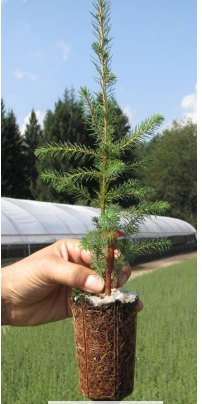
\includegraphics[width=0.35\textwidth]{plant_epinette.png}
	\caption{Plant d'épinette blanche. (Par Julie Gravel Grenier, Pépinière de Saint-Modeste)}
	\label{plant}	
	
\end{figure}

\subsection*{Plan expérimental}

L'expérience sera composée de trois traitements, un témoin (conditions environnementales optimales), un avec faible stress hydrique imposé et le dernier avec un stress hydrique plus intense avec quatre répétitions (en blocs) par traitement. Comme il s'agit de traitements d'arrosage, il ne serait pas pratique de constituer des blocs complets aléatoires avec chacun des plants. Les 35 plants de chacun des traitements seront donc placés côte-à-côte dans chaque bloc. Le niveau de sécheresse sera défini par la fréquence d'arrosage. Le témoin aura un arrosage quotidien, 2 arrosages par semaine seront effectués pour le faible stress et 1 arrosage par semaine pour le traitement de stress intense. Dans la serre les conditions environnementales seront contrôlées. Les principaux facteurs environnementaux qui seront contrôlés sont l'humidité du sol et la fréquence d'arrosage (précipitations). Les semis seront inclinés afin de les obliger à faire du bois de réaction d'un côté et du bois normal de l'autre. Le bois normal sera utilisé pour les analyses, ainsi nous nous affranchirons des effets du bois de flexion produit dans les premières années de la vie d'un arbre \citep{Telewski1989}. L'expérience sera réalisée sur une durée de deux ans. Après la première année, une partie des semis sera coupée et analysée.


\subsection*{Détermination de l'angle des microfibrilles}
L'angle des microfibrilles sera déterminé à l'aide d'un diffractomètre à rayon-X SilviScan-3 avec une résolution de 2 mm, soit la résolution maximale de l'appareil. Les échantillons d'arbres seront scannés de la moelle à l'écorce et la moyenne de l'angle des microfibrilles calculée sur un intervalle de 2 mm.
Les informations données par les profils de diffraction nous permettront d'avoir l'orientation moyenne des microfibrilles dans la couche S2 de la paroi cellulaire secondaire \citep{Evans1999}.

\subsection*{La masse volumique (densité)}

\begin{enumerate}
	 

\item \textbf{Préparation des échantillons}

La densité du bois sera mesurée à partir de coupes anatomiques dans le plan radial-tangentiel (ou transversal) du bois. Des cubes seront prélevés de la moelle à l'écorce. Nous allons saturer les cubes d'eau, et les laisser tremper dans l'eau pendant 48 heures. Les coupes seront recouvertes de safranine, puis trempées dans un mélange d'éthanol et d'eau distillée. Après coloration, les coupes seront placées sur des lames et des lamelles et laissées à sécher. Après séchage, des images prises à l'aide d'une caméra montée sur un microscope seront traitées à l'aide du logiciel Wincell. Le ratio de paroi cellulaire par rapport à l'espace occupé sera utilisé afin de d'estimer la masse volumique. \\

\item \textbf{Détermination de la masse volumique}

La méthode utilisée pour la détermination de la masse volumique est fondée sur l'hypothèse que la masse volumique des parois cellulaires ($\rho_{paroi}$) est homogène sur toutes leurs surfaces, avec une valeur allant de 1 à 1460 kg.m \textsuperscript{-3} selon les espèces et les études \citep{Decoux2004}. Ensuite l'équation suivante permet d'estimer la masse volumique: \\

\begin{equation}\label{eq:1}
\rho_{tracheide} = \rho_{paroi}\cdot\frac{A_{paroi}}{A_{tracheide}}
\end{equation}\\

Avec $\rho_{tracheide}$ qui représente la masse volumique de la surface radiale couverte par la trachéide (en g.dm$^{-3}$); $A_{paroi}$ représentant l'aire recouverte par la paroi de la trachéide (en m$^{2}$) et $A_{tracheide}$ l'aire recouverte par la trachéide entière (en m$^{2}$).\\

La détermination de la masse volumique par l'équation \ref{eq:1} considère que la paroi cellulaire est homogène. Or, le bois est formé de plusieurs constituants (cellulose, lignine, etc). Par conséquent, nous ferons également une mesure de la densité par densitomètre à rayon-X ce qui nous donnera une information complémentaire sur la densité.
\end{enumerate}

\subsection*{Détermination de la conductivité spécifique ($k_{s}$)}
La conductivité spécifique nous renseigne sur la réaction de l'arbre face à la sécheresse. C'est le rapport entre l’écoulement de l’eau et le gradient de pression responsable de cet écoulement, le tout par unité de surface \citep{Tyree1991}. Elle nous renseigne sur la perméabilité globale de la tige. Il faut souligner que la conductivité spécifique est une valeur théorique et elle ne prend en compte le fait que les caractéristiques des ponctuations influencent aussi l'écoulement de la sève \citep{Pothier1989}. %AA: pourquoi ne prendrais-tu pas des mesures similaires à celles de Pothier? On pourra en discuter à la soutenance
Elle reste malgré tout un bon moyen de comparaison de différents groupes (ex: traitements, familles etc).  Elle sera calculée à partir de l'équation suivante: \\

\begin{equation}\label{eq:2}
k_{s} = N\cdot \frac{\pi \cdot \rho_{w}}{128 \cdot \eta} \cdot <L>^{4}
\end{equation}\\

Avec $N$ qui représente la densité des trachéides (en m$^{-2}$); $\rho_{w}$ représentant la densité de l'eau (1 kg.m$^{-3}$); $\eta$ la viscosité de l'eau à 20  \textdegree C fluide (10$^{-3}$ Pa.s$^{-1}$) et $<L>^{4}$ la moyenne de l'ensemble des diamètres des trachéides puissance 4 (en m$^{4}$) ce qui permet de faire ressortir l'effet des lumens les plus larges \citep{Tyree1991}.


\subsection*{Analyses statistiques}
Les données récoltées après l'expérience seront traitées statistiquement pour déterminer la significativité des variations de la densité, l'angle des microfibrilles et de la conductivité du xylème entre les traitements et les clones. Dans cette analyse, nous mettrons en relation d'une part, les effets des traitements de sécheresse sur chacune des propriétés mesurées (la densité, l'angle des microfibrilles et la conductivité) et verrons dans quelle mesure une part significative de la variance est reliée aux différences entre les clones. D'autre part, les corrélations entre les changements de croissance induits par la sécheresse et les changements de densité, d'angle des microfibrilles et de conductivité seront évaluées. \\ 

Nous utiliserons des modèles linéaires mixtes pour le traitement de données pour les mêmes raisons que dans le premier chapitre. Les variables dépendantes seront la densité, l'angle des microfibrilles et la conductivité spécifique. Les variables à effet aléatoire seront le bloc . Les variables à effet fixe seront les trois niveaux de traitements et le clone. Le package nlme \citep{NLME2018} du logiciel R sera utilisé pour la construction de nos modèles linéaires mixtes. 

\section{Résultats attendus}
%\phantomsection\addcontentsline{toc}{section}{Résultats attendus}

Dans les résultats de cette expérience, on s'attend à une réaction à la sécheresse des arbres par groupes en fonction des clones. La réaction des clones peut être différente entre le témoin et les traitements et entre les différents traitements. Les arbres utilisent différentes stratégies de survie contre la sécheresse. \cite{Ambrose2015} ont mis en place une expérience en serre afin de comparer la physiologie et la croissance de deux espèces de séquoia, \textit{Sequoia sempervirens} (D. Don.) Endl. (coast redwood) et \textit{Sequoiadendron giganteum} (Lindl.) Buchh. (giant sequoia) soumises à une sécheresse progressive suivie d'une période de récupération. Les auteurs ont mesuré l'humidité du sol, les échanges gazeux des feuilles, l'embolie et la croissance entre le témoin et les traitements. Les résultats de l'étude ont montré des stratégies contrastées des deux espèces face à la sécheresse, mais aussi des différences intraspécifiques. Afin de s'adapter à la sécheresse, les arbres font des compromis qui sont à l'origine des stratégies d'adaptation. Chaque stratégie présente des avantages et des  inconvénients. Les arbres peuvent choisir (1) la fermeture des stomates pour réduire l'évapotranspiration \citep{Martinez-Sancho2017}, (2) changer l'anatomie des cellules pour produire une paroi plus épaisse et plus dense ou (3) produire une paroi avec un angle des microfibrilles plus faible et donc plus rigide. Dans le cas de notre étude on peut donc s'attendre à une différence de stratégie d'adaptation entre nos clones face au stress de sécheresse. En fonction des stratégies utilisées par les clones, on s'attend à une relation entre la conductivité et les propriétés du bois. En effet, les arbres qui produiront une paroi plus épaisse auront des lumens plus petits et donc une conductivité plus faible. Dans ces conditions, nous pourrons établir un lien entre la conductivité, la densité du bois, l'angle des microfibrilles et la sécheresse. \\ %AA: C'est une très bonne explication des résultats attendus, sauf que tu n'as pas mis les clones en évidence dans ton analyse statistique. Je te l'ai placé en effet aléatoire, ce qui ne te permettra pas d'aller aussi loin que tu le dis. Tu peux le replacer dans les effets fixes. On pourra en rediscuter le jour de la présentation.


\section{Conclusion}
%\phantomsection\addcontentsline{toc}{section}{Conclusion}

Cette expérience permettra de mieux comprendre l'impact de différents niveaux de sécheresse sur les propriétés du bois. Ainsi, nous pourrons mieux comprendre la variabilité des mécanismes d'adaptation à la sécheresse liée aux clones. Chaque stratégie d'adaptation à la sécheresse a un coût pour l'arbre. De ce fait, nous pensons qu'il n'est pas avantageux pour l'arbre d'associer plusieurs stratégies. Si notre hypothèse est vérifiée, les clones auront des stratégies différentes et donc une variation des propriétés du bois et de la conductivité liée à la stratégie. Les clones dont la stratégie d'adaptation à la sécheresse permet d'avoir les meilleures propriétés seront considérés intéressant pour le reboisement et l'amélioration génétique.\\

Cette seconde partie du projet servira à faire une sélection des clones ou familles qui serviront au reboisement et aussi à l'amélioration génétique. L'utilisation de la densité et de la largeur des cernes pour prédire l'impact du climat sur les propriétés bois a ses limites. Une nouvelle méthode (la signature isotopique) fondée sur une mesure à partir de la cellulose du bois est maintenant utilisée afin d'avoir des informations complémentaires. Il a été mis en évidence dans des études antérieures qu'il existe une relation entre la proportion d'isotopes stables (\Ctreize et \Odixhuit) et les conditions environnementales. Cependant, l'effet de la famille sur la signature isotopique du bois en lien avec le climat est peu connu.  Par conséquent, dans le chapitre 3, nous prendrons en compte ce nouveau facteur en plus de ceux étudiés dans les deux chapitres précédents. Ce chapitre permettra l'identification des familles aux caractéristiques les plus avantageuses face à la sécheresse et la caractérisation du stress climatique au niveau du bois par la signature isotopique.


\chapter{Chapitre 3: Quantification des effets du climat sur la variation de la proportion d'isotopes stables (\Ctreize et \Odixhuit) face au climat et entre familles chez \textit{Picea glauca}}

Les objectifs de ce chapitre sont (1) de quantifier les effets des conditions météorologiques sur la proportion d'isotopes stables lourds dans la cellulose du bois et (2) de déterminer dans quelle mesure cette proportion peut varier entre les familles analysées. %AA: c'est OK comme objectifs, mais idéalement ton dernier chapitre devrait être utilisé pour rassembler les autres et boucler la boucle. Pour y arriver, il faudrait idéalement que tu fasses le lien avec les propriétés du bois. 

\section{Matériel et méthode}
%\phantomsection\addcontentsline{toc}{section}{Matériel et méthode}

\subsection*{Site et matériel}
Le matériel utilisé pour cette partie de notre étude est le même que celui décrit dans le premier chapitre (voir \ref{matériel}).  

%\subsection*{Détermination de la densité}
%La méthode de détermination de la densité est la même que celle utilisée dans le premier chapitre (voir \ref{densité}). %AA: tu ne parles pas de la densité, ni dans les objectifs, ni dans les analyses statistiques...

\subsection*{Mesures isotopiques}
Les mesures isotopiques sont effectuées à partir de cellulose qui est le principal composant du bois. Nous ferons une série de coupes d'une épaisseur de 1 millimètre dans quatre directions cardinales principales. Les coupes seront prélevées l'aide du microtome par séquence du bois initial au bois final. Le bois des quatre directions de chaque échantillon seront mélangés, puis broyé pour extraire l'alpha-cellulose. Après l'extraction de l'alpha-cellulose, les échantillons seront envoyés au laboratoire "Delta Lab" de la commission géologique du Canada où les proportions de \Ctreize et \Odixhuit seront mesurées.

\subsection*{Analyses statistiques}
Les données seront traitées statistiquement pour déterminer la variabilité de la composition isotopique de la cellulose qui est associée aux conditions environnementales. Dans cette analyse, nous mettrons en relation d'une part, la signature isotopique du bois avec les facteurs environnementaux et d'autre part, la variabilité de la signature isotopes qui est liée aux familles. \\

Comme précédemment, nous utiliserons des modèles linéaires mixtes pour le traitement des données. La variable indépendante sera la signature isotopique. Les variables à effet aléatoire sont le site, le bloc et l'arbre. Les variables à effet fixe sont les précipitations, les indices de sécheresse et la famille. Le logiciel R et plus spécifiquement le package nlme sera utilisé pour la construction de nos différents modèles. 

\section{Résultats attendus}
%\phantomsection\addcontentsline{toc}{section}{Résultats attendus}

Dans ce chapitre, on s'attend d'une part, à une relation entre la composition isotopique du bois et les autres propriétés du bois (densité, largeur des cernes et angle des microfibrilles) et d'autre part, à une relation entre la signature isotopique et les variations climatiques comme d'autres études l'ont déjà montré. Ensuite, nous nous attendons à une composition isotopique similaire chez les individus issus de la même famille.\\

On s'attend à des résultats similaires à ceux qu'on trouve dans la littérature. Dans certaines études, un lien a déjà été observé entre la densité du bois, l'angle des microfibrilles, \Ctreize et la sécheresse. C'est le cas de \cite{Drew2009} qui ont trouvé une augmentation de ces propriétés du bois et la sécheresse. En plus, de ces résultats une relation entre la variation de ces facteurs et la famille pourra être observée.  

\section{Conclusion}
%\phantomsection\addcontentsline{toc}{section}{Conclusion}

Les résultats de ce chapitre permettront de mettre en évidence le lien potentiel entre la variation de la signature isotopique et les propriétés du bois (densité, largeur des cernes) en fonction des conditions climatiques. Si une partie de la variation de la signature isotopique est due à la famille, elle sera quantifiée et permettra une meilleure isolation du climat comme facteur explicatif de la variation de la proportion d'isotopes stables (\Ctreize et \Odixhuit) dans le bois.\\

Les analyses isotopiques proviennent de la cellulose, ce qui augmente leur précision comparée à d'autres analyses. Ainsi, si on obtient les résultats escomptés, les analyses isotopiques permettront d'anticiper l'impact du climat futur sur la production du bois. L'utilisation de la famille comme facteur explicatif de la variation isotopique peut réduire le nombre d'échantillons dans le cas des forêts constituées de population issues de sélection génétique. % Je ne saisis pas cette dernière affirmation

\clearpage % passer à la page suivante

\chapter*{Conclusions et perspectives}
\phantomsection\addcontentsline{toc}{chapter}{Conclusions et perspectives}

L'amélioration génétique a longtemps servi à l'augmentation de la production du bois sans prendre en compte sa qualité. La qualité du bois est de plus en plus considérée dans les programmes d'amélioration. Alors que le bois est davantage utilisé pour substituer au  béton ou à l'acier dans la société d'aujourd'hui, il est d'autant plus important qu'il soit de qualité. La possibilité de substituer certains matériaux par le bois est l'une des solutions pour freiner les changements climatiques du fait que le bois contribue au stockage du carbone. La prédiction des effets potentiels des changements climatiques sur la production et la qualité du bois permet d'anticiper ceux-ci et d'adapter le choix des semis utilisés pour le reboisement des forêts. \\

Cette thèse donnera des outils pour anticiper les effets potentiels des variations climatiques sur la qualité du bois. La caractérisation de l'impact des conditions météorologiques sur les propriétés telles que la densité, la largeur des annaux de croissance annuelle, l'angle des microfibrilles et la signature isotopique du bois permet une sélection des familles aux stratégies de résistance au stress les plus avantageuses. L'amélioration génétique sera alors un outil efficace pour une production optimale de bois de bonne qualité. Il existe une corrélation positive entre la densité et la sécheresse, contrairement à la conductivité qui semble corrélée négativement au stress hydrique. Certaines familles d'arbres peuvent avoir une stratégie optimale pour la production de bois de qualité en conditions de stress. Ces familles auront alors un potentiel intéressant pour le reboisement dans un contexte de climat changeant. \\

Si une corrélation est observée entre la densité, la largeur des cernes, l'angle des microfibrilles, la sécheresse et la proportion d'isotopes stables lourds (\Ctreize et \Odixhuit) alors la signature isotopique, de par sa précision, pourra être utilisée afin d'avoir des informations à la fois sur les conditions climatiques et sur les différentes propriétés du bois. L'interdisciplinarité de cette thèse permettra de contribuer à l'avancée des connaissances fondamentales de la science et aussi l'application des découvertes scientifiques par la sélection des familles pour le reboisement des forêts futures. \\

\clearpage
	
\begin{figure}
	\includegraphics[width=1.1\columnwidth]{Calendrier.pdf}
	\caption{Calendrier prévisionnel de la thèse}
	\label{fig:calendrier}
	\end{figure}


\bibliography{bibliographie}
\bibliographystyle{apalike}
\end{document}